% move all configuration stuff into one file so we can focus on the content
\documentclass[aspectratio=169,hyperref={pdfpagelabels=false,colorlinks=true,linkcolor=white,urlcolor=blue},t]{beamer}

%%%%%%%%%%%%%%%%%%%%%%%%%%%%%%%%%%%%%%%%%%%%%%%%%%%%%%%%%%%%%%%%%%%%%%%%%%%%%%%%%%
%%%%%%%%%%%%%%%%%%%%%%%%%%%%%%%%%%%%%%%%%%%%%%%%%%%%%%%%%%%%%%%%%%%%%%%%%%%%%%%%%%
% packages
\usepackage{pict2e}
\usepackage{epic}
\usepackage{amsmath,amsfonts,amssymb}
\usepackage{units}
\usepackage{fancybox}
\usepackage[absolute,overlay]{textpos} 
\usepackage{media9} % avi2flv: "C:\Program Files\ffmpeg\bin\ffmpeg.exe" -i TuneFreqFilterbank.avi -b 600k -s 441x324 -r 15 -acodec copy TuneFreqFilterbank.flv
\usepackage{animate}
\usepackage{gensymb}
\usepackage{multirow}
\usepackage{silence}
\usepackage[backend=bibtex,style=ieee]{biblatex}
\AtEveryCitekey{\iffootnote{\tiny}{}}
\addbibresource{references}

%%%%%%%%%%%%%%%%%%%%%%%%%%%%%%%%%%%%%%%%%%%%%%%%%%%%%%%%%%%%%%%%%%%%%%%%%%%%%%%%%%
%%%%%%%%%%%%%%%%%%%%%%%%%%%%%%%%%%%%%%%%%%%%%%%%%%%%%%%%%%%%%%%%%%%%%%%%%%%%%%%%%%
% relative paths
\graphicspath{{graph/}}


%%%%%%%%%%%%%%%%%%%%%%%%%%%%%%%%%%%%%%%%%%%%%%%%%%%%%%%%%%%%%%%%%%%%%%%%%%%%%%%%%%
%%%%%%%%%%%%%%%%%%%%%%%%%%%%%%%%%%%%%%%%%%%%%%%%%%%%%%%%%%%%%%%%%%%%%%%%%%%%%%%%%%
% units
\setlength{\unitlength}{1mm}

%%%%%%%%%%%%%%%%%%%%%%%%%%%%%%%%%%%%%%%%%%%%%%%%%%%%%%%%%%%%%%%%%%%%%%%%%%%%%%%%%%
%%%%%%%%%%%%%%%%%%%%%%%%%%%%%%%%%%%%%%%%%%%%%%%%%%%%%%%%%%%%%%%%%%%%%%%%%%%%%%%%%%
% theme & layout
\usetheme{Frankfurt}
\beamertemplatenavigationsymbolsempty
%\setbeamertemplate{frametitle}[smoothbars theme]
\setbeamertemplate{frametitle}
{
    \begin{beamercolorbox}[ht=1.8em,wd=\paperwidth]{frametitle}
        \vspace{-.1em}%
        \hspace{.2em}{\strut\insertframetitle\strut}
        
        \hspace{.2em}\small\strut\insertframesubtitle\strut
        %\hfill
        %
\includegraphics[height=.8cm,keepaspectratio]{CenterMusicTechnology-solid-2lines-white-CoAtag}
        
    \end{beamercolorbox}
    \begin{textblock*}{100mm}(11.6cm,.7cm)
        \includegraphics[height=.8cm,keepaspectratio]{logo_GTCMT_black}
    \end{textblock*}
}

% set this to ensure bulletpoints without subsections
\usepackage{remreset}
\makeatletter
\@removefromreset{subsection}{section}
\makeatother
\setcounter{subsection}{1}

%---------------------------------------------------------------------------------
% appearance
\setbeamercolor{structure}{fg=gtgold}
\setbeamercovered{transparent} %invisible
\setbeamercolor{bibliography entry author}{fg=black}
\setbeamercolor*{bibliography entry title}{fg=black}
\setbeamercolor*{bibliography entry note}{fg=black}

%\usepackage{pgfpages}
%\setbeameroption{show notes}
%\setbeameroption{show notes on second screen=right}
%---------------------------------------------------------------------------------
% fontsize
\let\Tiny=\tiny

%%%%%%%%%%%%%%%%%%%%%%%%%%%%%%%%%%%%%%%%%%%%%%%%%%%%%%%%%%%%%%%%%%%%%%%%%%%%%%%%%%
%%%%%%%%%%%%%%%%%%%%%%%%%%%%%%%%%%%%%%%%%%%%%%%%%%%%%%%%%%%%%%%%%%%%%%%%%%%%%%%%%%
% warnings
\pdfsuppresswarningpagegroup=1
\WarningFilter{biblatex}{Patching footnotes failed}
\WarningFilter{latexfont}{Font shape}
\WarningFilter{latexfont}{Some font shapes}
\WarningFilter{gensymb}{Not defining}



\subtitle{Part 8.1: Alignment}

%%%%%%%%%%%%%%%%%%%%%%%%%%%%%%%%%%%%%%%%%%%%%%%%%%%%%%%%%%%%%%%%%%%%%%%%%%%%
\begin{document}
    % generate title page
	

\begin{frame}
    \titlepage
    %\vspace{-5mm}
    \begin{flushright}
        \href{http://www.gtcmt.gatech.edu}{\includegraphics[height=.8cm,keepaspectratio]{logo_GTCMT_black}}
    \end{flushright}
\end{frame}


    \section[overview]{lecture overview}
        \begin{frame}{temporal analysis}{overview}
            \begin{itemize}
                \item   \textbf{text book}  
                    \begin{itemize}
                        \item   \href{http://ieeexplore.ieee.org/xpl/articleDetails.jsp?tp=&arnumber=6331124&}{\underline{\textit{Chapter 7: Alignment} (pp.~139--150)}}
                    \end{itemize}
                \item   \textbf{sources}: slides (latex) \& Matlab  
                    \begin{itemize}
                        \item   \href{https://github.com/alexanderlerch/ACA-Slides}{\underline{github repository}}
                    \end{itemize}
                \bigskip
                \item<2->   \textbf{lecture content}
                    \begin{itemize}
                        \item<2->   Dynamic Time Warping
                        \item<3->   Audio-to-Audio Alignment
                        \item<4->   Audio-to-Score Alignment
                    \end{itemize}
            \end{itemize}
        \end{frame}

    \section[intro]{introduction}
        \begin{frame}{alignment}{introduction}
            \begin{itemize}
                \only<1>{\item   align/\textbf{synchronize two sequences}
                    \begin{itemize}
                        \item	\textit{similar} musical content
                        \item	\textit{different} tempo and timing
                            \begin{itemize}
                                \item[]	$A(n_\mathrm{A})\quad n_\mathrm{A} \in [0;\mathcal{N}_\mathrm{A}-1]$
                                \item[]	$B(n_\mathrm{B})\quad n_\mathrm{B} \in [0;\mathcal{N}_\mathrm{B}-1]$
                            \end{itemize}
                    \end{itemize}}
                \only<1>{
                    \vspace{-5mm}
                    \figwithmatlab{SequenceAlignment}
                }
            \item<2->   \textbf{processing steps}
                \begin{enumerate}
                    \item   extract suitable features (pitch chroma, timbre features, ...)
                    \item<3->	compute distance matrix $\mat{D}_{\mathrm{AB}}(n_\mathrm{A},n_\mathrm{B})$
                        \only<3>{
                        
                            \figwithmatlab{SimMatrix}
                            }
                    \item<4->	DTW: compute alignment path $\vec{P}(n_\mathrm{P})$ with $n_\mathrm{P} \in
                [0;\mathcal{N}_{\mathrm{P}}-1]$
                        \begin{itemize}
                            \item[$\Rightarrow$]	minimal \textit{overall} distance
                        \end{itemize}
                    \item<5->   align sequences using dynamic time stretching
                \end{enumerate}
            \end{itemize}
        \end{frame}
    \section[DTW]{dynamic time warping}
        \begin{frame}{alignment}{dynamic time warping (DTW)}
            \begin{itemize}
                \item   dynamic programming technique
                \item   time is warped non-linearily to match sequences
                \item   finds optimal match between two sequences given a cost function
                \item   the overall cost indicates the overall distance between the sequences
            \end{itemize}
        \end{frame}
        \begin{frame}{alignment}{DTW: example}
            \figwithmatlab{Dtw}
        \end{frame}
        \begin{frame}{alignment}{DTW: path conditions 1/2}
            \begin{itemize}
                    \item	\textbf{boundaries}: covers both $A,B$ from beginning to end
                            \begin{eqnarray*}
                                \vec{P}(0) 		&=& [0, 0] \\
                                \vec{P}(\mathcal{N}_{\mathrm{P}}-1) 	&=& [\mathcal{N}_\mathrm{A}-1, \mathcal{N}_\mathrm{B}-1] 
                            \end{eqnarray*}
                    \pause
                    \item	\textbf{causality}: only forward movement
                            \begin{eqnarray*}
                                n_\mathrm{A}\big|_{\vec{P}(n_\mathrm{P})} \leq n_\mathrm{A}\big|_{\vec{P}(n_\mathrm{P}+1)} \\ 
                                n_\mathrm{B}\big|_{\vec{P}(n_\mathrm{P})} \leq n_\mathrm{B}\big|_{\vec{P}(n_\mathrm{P}+1)} 
                            \end{eqnarray*}
                    \pause
                    \item	\textbf{continuity}: no jumps
                            \begin{eqnarray*}
                                n_\mathrm{A}\big|_{\vec{P}(n_\mathrm{P}+1)} \leq (n_\mathrm{A}+1)\big|_{\vec{P}(n_\mathrm{P})} \\ 
                                n_\mathrm{B}\big|_{\vec{P}(n_\mathrm{P}+1)} \leq (n_\mathrm{B}+1)\big|_{\vec{P}(n_\mathrm{P})} 
                            \end{eqnarray*}
            \end{itemize}
        \end{frame}
        \begin{frame}{alignment}{DTW: path conditions 2/2}
                \begin{figure}
                    \begin{footnotesize}
				\begin{picture}(30,30)
                    \setlength\fboxsep{0pt}
					\setcounter{iXOffset}{10}
					\setcounter{iXBlockSize}{5}
					\setcounter{iYBlockSize}{5}
					%\setcounter{iYBlockSizeDiv2}{2}
					%\setcounter{iDistance}{8}

                    \setcounter{i}{1}
                    \whiledo{\value{i}<5}
					{
                        \setcounter{iYOffset}{10}
                        \setcounter{j}{1}
                        \whiledo{\value{j}<5}
                        {
                            \put(\value{iXOffset}, \value{iYOffset})
                                {\framebox(\value{iXBlockSize}, \value{iYBlockSize})}
                            \addtocounter{iYOffset}{\value{iYBlockSize}}
                            \stepcounter{j}
                        }
                        \addtocounter{iXOffset}{\value{iXBlockSize}}
                        \stepcounter{i}
                    }
                    \setcounter{iXOffset}{12}
                    \setcounter{iYOffset}{26}
                    \setcounter{i}{1}
                    \whiledo{\value{i}<5}
					{
                        \put(\value{iXOffset}, 6)
                            {\arabic{i}}
                        \put(6,\value{iYOffset})
                            {\arabic{i}}
                        \addtocounter{iYOffset}{-\value{iYBlockSize}}
                        \addtocounter{iXOffset}{\value{iXBlockSize}}
                        \stepcounter{i}
                    }
					\put(20, 3)
						{\text{$n_\mathrm{A}$}}
					\put(0, 20)
						{\text{$n_\mathrm{B}$}}
					\put(15, 20)
                        {\colorbox{gray!40}{\framebox(\value{iXBlockSize}, \value{iYBlockSize}){}}}
					\put(17.5, 22.5)
                        {{\vector(1,0){5}}}
					\put(17.5, 22.5)
                        {{\vector(1,-1){5}}}
					\put(17.5, 22.5)
                        {{\vector(0,-1){5}}}
				\end{picture}
\end{footnotesize}

                \end{figure}
                \pause
                \question{what is the minimum/maximum path length}
                    \begin{equation*}
                        \mathcal{N}_\mathrm{P, min} = \max(\mathcal{N}_\mathrm{A}, \mathcal{N}_\mathrm{B})
                    \end{equation*}
                    \begin{equation*}
                        \mathcal{N}_\mathrm{P, max} = \mathcal{N}_\mathrm{A} + \mathcal{N}_\mathrm{B} - 2
                    \end{equation*}
        \end{frame}
        \begin{frame}{alignment}{DTW: overall cost}
            \begin{itemize}
                \item	every path has an \textit{overall cost}
                    \begin{equation*}
                        \mathfrak{C}_{\mathrm{AB}}(j) = \sum\limits_{n_\mathrm{P}= 0}^{\mathcal{N}_{\mathrm{P}}-1}{\mat{D}\big(\vec{P}_j(n_\mathrm{P})\big)} 
                    \end{equation*}
                \item<2->	\textit{optimal} path minimizes the overall cost
                    \begin{eqnarray*}
                        \mathfrak{C}_{\mathrm{AB},min} &=& \min\limits_{\forall j}\big(\mathfrak{C}_{\mathrm{AB}}(j)\big) \\
                        j_\mathrm{opt} 				&=& \argmin\limits_{\forall j}\big(\mathfrak{C}_{\mathrm{AB}}(j)\big) 
                    \end{eqnarray*}
                \item[$\Rightarrow$]<2-> stay in the 'valleys' of distance matrix
                \item<3->	how to determine the optimal path?
            \end{itemize}
        \end{frame}
        \begin{frame}{alignment}{DTW: accumulated cost 1/2}
            accumulated cost: \textit{cost matrix}
                \begin{equation*}\label{eq:acccost}
                            \mat{C}_{\mathrm{AB}}(n_\mathrm{A},n_\mathrm{B}) = \mat{D}_{\mathrm{AB}}(n_\mathrm{A},n_\mathrm{B}) + \min\left\{
                                                    \begin{array}{llr} 
                                                        \mat{C}_{\mathrm{AB}}(n_\mathrm{A}-1, n_\mathrm{B}-1)\\
                                                        \mat{C}_{\mathrm{AB}}(n_\mathrm{A}-1, n_\mathrm{B}) \\
                                                        \mat{C}_{\mathrm{AB}}(n_\mathrm{A},	n_\mathrm{B}-1)
                                                    \end{array} 
                                                    \right. 
                \end{equation*}
                \begin{itemize}
                    \item	initialization
                        \begin{equation*}
                            \mat{C}_{\mathrm{AB}}(0,0) 	= \mat{D}_{\mathrm{AB}}(0,0) 
                        \end{equation*}
                \end{itemize}
                \begin{figure}
                    \begin{footnotesize}
				\begin{picture}(30,30)
                    \setlength\fboxsep{0pt}
					\setcounter{iXOffset}{10}
					\setcounter{iXBlockSize}{5}
					\setcounter{iYBlockSize}{5}
					%\setcounter{iYBlockSizeDiv2}{2}
					%\setcounter{iDistance}{8}

                    \setcounter{i}{1}
                    \whiledo{\value{i}<5}
					{
                        \setcounter{iYOffset}{10}
                        \setcounter{j}{1}
                        \whiledo{\value{j}<5}
                        {
                            \put(\value{iXOffset}, \value{iYOffset})
                                {\framebox(\value{iXBlockSize}, \value{iYBlockSize})}
                            \addtocounter{iYOffset}{\value{iYBlockSize}}
                            \stepcounter{j}
                        }
                        \addtocounter{iXOffset}{\value{iXBlockSize}}
                        \stepcounter{i}
                    }
                    \setcounter{iXOffset}{12}
                    \setcounter{iYOffset}{26}
                    \setcounter{i}{1}
                    \whiledo{\value{i}<5}
					{
                        \put(\value{iXOffset}, 6)
                            {\arabic{i}}
                        \put(6,\value{iYOffset})
                            {\arabic{i}}
                        \addtocounter{iYOffset}{-\value{iYBlockSize}}
                        \addtocounter{iXOffset}{\value{iXBlockSize}}
                        \stepcounter{i}
                    }
					\put(20, 3)
						{\text{$n_\mathrm{A}$}}
					\put(0, 20)
						{\text{$n_\mathrm{B}$}}
					\put(15, 20)
                        {\colorbox{gray!40}{\framebox(\value{iXBlockSize}, \value{iYBlockSize}){}}}
					\put(17.5, 22.5)
                        {{\vector(1,0){5}}}
					\put(17.5, 22.5)
                        {{\vector(1,-1){5}}}
					\put(17.5, 22.5)
                        {{\vector(0,-1){5}}}
				\end{picture}
\end{footnotesize}

                \end{figure}
        \end{frame}
        \begin{frame}{alignment}{DTW: accumulated cost 2/2}
            \figwithmatlab{DtwCost}
        \end{frame}
        \begin{frame}{alignment}{DTW: algorithm description 1/2}
                \begin{itemize}
                    \item	\textbf{initialization}:
                        \begin{footnotesize}
                            \begin{equation*}
                                \mat{C}_{\mathrm{AB}}(0,0) = \mat{D}_{\mathrm{AB}}(0,0) ,
                                \mat{C}_{\mathrm{AB}}(n_\mathrm{A},-1) = \infty ,
                                \mat{C}_{\mathrm{AB}}(-1,n_\mathrm{B}) = \infty \nonumber
                            \end{equation*}
                        \end{footnotesize}
                    \item<2->	\textbf{recursion}:
                        \begin{footnotesize}
                            \begin{eqnarray*}
                                \mat{C}_{\mathrm{AB}}(n_\mathrm{A},n_\mathrm{B}) &=& \mat{D}_{\mathrm{AB}}(n_\mathrm{A},n_\mathrm{B}) + \min\left\{
                                                            \begin{array}{l} 
                                                                \mat{C}_{\mathrm{AB}}(n_\mathrm{A}-1, n_\mathrm{B}-1)\\
                                                                \mat{C}_{\mathrm{AB}}(n_\mathrm{A}-1, n_\mathrm{B}) \\
                                                                \mat{C}_{\mathrm{AB}}(n_\mathrm{A},	n_\mathrm{B}-1)
                                                            \end{array} 
                                                            \right. \\
                                j &=& \argmin\left\{
                                                            \begin{array}{l} 
                                                                \mat{C}_{\mathrm{AB}}(n_\mathrm{A}-1, n_\mathrm{B}-1)\\
                                                                \mat{C}_{\mathrm{AB}}(n_\mathrm{A}-1, n_\mathrm{B}) \\
                                                                \mat{C}_{\mathrm{AB}}(n_\mathrm{A},	n_\mathrm{B}-1)
                                                            \end{array} 
                                                            \right. \\
                                \Delta\vec{P}(n_\mathrm{A},n_\mathrm{B}) &=& \left\{ 
                                                            \begin{array}{ll} 
                                                              [-1, -1] &\mbox{if }	j = 0 \\{} 
                                                              [-1, 0] &\mbox{if }	j = 1 \\{}
                                                              [0, -1] &\mbox{if }	j = 2  
                                                            \end{array} 
                                                            \right.
                            \end{eqnarray*}
                        \end{footnotesize}
                \end{itemize}
        \end{frame}
        \begin{frame}{alignment}{DTW: algorithm description 2/2}
                \begin{itemize}
                    \item	\textbf{termination}:
                        \begin{footnotesize}
                            \begin{equation*}
                                n_\mathrm{A}= \mathcal{N}_\mathrm{A}-1 \wedge n_\mathrm{B} = \mathcal{N}_\mathrm{B}-1 
                            \end{equation*}
                        \end{footnotesize}
                    \bigskip
                    \item<2->	\textbf{path backtracking}:
                        \begin{footnotesize}
                            \begin{equation*}
                                \vec{P}(n_\mathrm{P}) = \vec{P}(n_\mathrm{P}+1) + \Delta\vec{P}\big(\vec{P}(n_\mathrm{P}+1)\big), \;n_\mathrm{P} = \mathcal{N}_{\mathrm{P}}-2, \mathcal{N}_{\mathrm{P}}-3,\ldots, 0 \nonumber
                            \end{equation*}
                        \end{footnotesize}
                \end{itemize}
        \end{frame}
        \begin{frame}{alignment}{DTW: example}
            \question{compute distance matrix, cost matrix, and DTW path}
                    \begin{eqnarray*}
                        A &=& [1,\ 2,\ 3,\ 0] ,\nonumber\\
                        B &=& [1,\ 0,\ 2,\ 3,\ 1] ,\nonumber
                    \end{eqnarray*}
                    \pause
                    \begin{equation*}
                    \mat{D}_{\mathrm{AB}} =   \left[ 
                                    \begin{array}{cccc}
                                    0							&	\textcolor[gray]{0.6}{1}	&	\textcolor[gray]{0.6}{2}	&	\textcolor[gray]{0.6}{1}\\
                                    1							&	\textcolor[gray]{0.6}{2}	&	\textcolor[gray]{0.6}{3}	&	\textcolor[gray]{0.6}{0}\\
                                    \textcolor[gray]{0.6}{1}	&	0 							&	\textcolor[gray]{0.6}{1}	&	\textcolor[gray]{0.6}{2}\\
                                    \textcolor[gray]{0.6}{2}	&	\textcolor[gray]{0.6}{1}	&	0							&	\textcolor[gray]{0.6}{3}\\
                                    \textcolor[gray]{0.6}{0}	&	\textcolor[gray]{0.6}{1}	&	\textcolor[gray]{0.6}{2}	&	1\\
                                \end{array}  
                            \right]  
                    \end{equation*}
                    
        \end{frame}
        \begin{frame}{alignment}{DTW: variants}
            \begin{itemize}
                \item	transition weights: favor specific path directions
                    \begin{footnotesize}
                        \begin{equation*}
                            \mat{C}_{\mathrm{AB}}(n_\mathrm{A},n_\mathrm{B}) = \min\left\{
                                                    \begin{array}{lll} 
                                                    \mat{C}_{\mathrm{AB}}(n_\mathrm{A}-1,n_\mathrm{B}-1)	&+& \lambda_\mathrm{d}\cdot\mat{D}_{\mathrm{AB}}(n_\mathrm{A},n_\mathrm{B})\\
                                                    \mat{C}_{\mathrm{AB}}(n_\mathrm{A}-1,n_\mathrm{B}) 	&+& \lambda_\mathrm{v}\cdot\mat{D}_{\mathrm{AB}}(n_\mathrm{A},n_\mathrm{B})\\
                                                    \mat{C}_{\mathrm{AB}}(n_\mathrm{A},n_\mathrm{B}-1) 	&+& \lambda_\mathrm{h}\cdot\mat{D}_{\mathrm{AB}}(n_\mathrm{A},n_\mathrm{B})
                                                    \end{array} 
                                                    \right.\nonumber
                        \end{equation*}
                    \end{footnotesize}
                \item<2->	step types
                \begin{figure}
                    \begin{footnotesize}
				\begin{picture}(50,30)
                    \setlength\fboxsep{0pt}
					
					\setcounter{iXBlockSize}{5}
					\setcounter{iYBlockSize}{5}
					%\setcounter{iYBlockSizeDiv2}{2}
					%\setcounter{iDistance}{8}

                    \setcounter{i}{1}
                    \setcounter{iXOffset}{0}
                    \whiledo{\value{i}<5}
					{
                        \setcounter{iYOffset}{0}
                        \setcounter{j}{1}
                        \whiledo{\value{j}<5}
                        {
                            \put(\value{iXOffset}, \value{iYOffset})
                                {\framebox(\value{iXBlockSize}, \value{iYBlockSize})}
                            \addtocounter{iYOffset}{\value{iYBlockSize}}
                            \stepcounter{j}
                        }
                        \addtocounter{iXOffset}{\value{iXBlockSize}}
                        \stepcounter{i}
                    }
					\put(5, 10)
                        {\colorbox{gray!40}{\framebox(\value{iXBlockSize}, \value{iYBlockSize}){}}}
					\put(7.5, 12.5)
                        {{\vector(2,-1){10}}}
					\put(7.5, 12.5)
                        {{\vector(1,-1){5}}}
					\put(7.5, 12.5)
                        {{\vector(1,-2){5}}}

                    \setcounter{i}{1}
                    \setcounter{iXOffset}{25}
                    \whiledo{\value{i}<5}
					{
                        \setcounter{iYOffset}{0}
                        \setcounter{j}{1}
                        \whiledo{\value{j}<5}
                        {
                            \put(\value{iXOffset}, \value{iYOffset})
                                {\framebox(\value{iXBlockSize}, \value{iYBlockSize})}
                            \addtocounter{iYOffset}{\value{iYBlockSize}}
                            \stepcounter{j}
                        }
                        \addtocounter{iXOffset}{\value{iXBlockSize}}
                        \stepcounter{i}
                    }
					\put(30, 10)
                        {\colorbox{gray!40}{\framebox(\value{iXBlockSize}, \value{iYBlockSize}){}}}
					\put(32.5, 12.5)
                        {{\line(1,0){5}}}
					\put(32.5, 12.5)
                        {{\vector(1,-1){5}}}
					\put(37.5, 12.5)
                        {{\vector(1,-1){5}}}
					\put(32.5, 7.5)
                        {{\vector(1,-1){5}}}
					\put(32.5, 12.5)
                        {{\line(0,-1){5}}}
				\end{picture}
\end{footnotesize}

                \end{figure}
                
            \end{itemize}
        \end{frame}
        \begin{frame}{alignment}{DTW: optimization}
            \vspace{-3mm}
            \begin{itemize}
                \item \textbf{problem}:  distance matrix dimensions  $\mathcal{N}_\mathrm{A}\cdot \mathcal{N}_\mathrm{B}$
                \item[$\Rightarrow$] DTW \textit{inefficient} for long sequences 
                    \begin{itemize}
                        \item	high memory requirements
                        \item	large number of operations
                    \end{itemize}
                \item<2-> \textbf{optimizations}:  
                    \begin{enumerate}
                        \item	maximum time and tempo deviation
                        \item<3->	sliding window \footfullcite{dixon_match:_2005}
                        \item<4->	multi-scale DTW (several downsampled iterations)
                    \end{enumerate}
            \end{itemize}
            \only<2>{
                \figwithmatlab{DtwConstraints}
            }
            \only<3>{
                \begin{figure}
                    \centerline{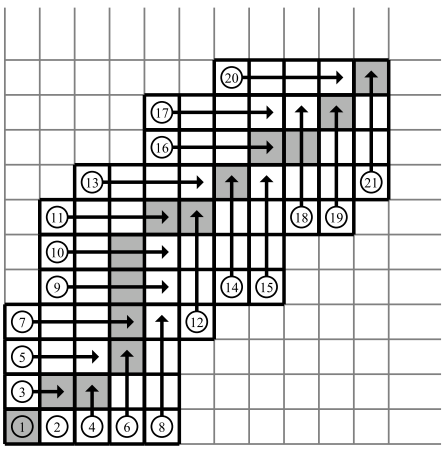
\includegraphics[scale=.2]{graph/dtw_match}}
                \end{figure}
            }
        \end{frame}

    \section[A2A]{Audio to audio alignment}
        \begin{frame}{audio-to-audio alignment}{introduction}
            \begin{itemize}
                \item	\textbf{objective}
                    \begin{itemize}
                        \item	align two sequences of audio
                    \end{itemize}
                \bigskip
                \item<2->	\textbf{use cases}
                    \begin{itemize}
                        \item	\textit{quick browsing} for certain parts in recordings
                        \item	\textit{timing adjustment} (backing vocals, loops, \ldots)
                        \item	\textit{automated dubbing}
                        \item	\textit{musicological analysis} (timing of several performances)
                    \end{itemize}
                \bigskip
                \item<3->	\textbf{processing steps}
                    \begin{itemize}
                        \item	extract suitable features
                        \item	compute distance matrix
                        \item	compute alignment path
                    \end{itemize}
            \end{itemize}
        \end{frame}

        \begin{frame}{audio-to-audio alignment}{features}
            \only<1-2>{
                \begin{itemize}
                    \item	\textbf{use case examples}
                        \begin{itemize}
                            \item	\textbf{quick browsing} --- find the same part across files\\
                                $\Rightarrow$ use \textit{pitch based} features
                            \item	\textbf{timing adjustment} --- backing vocals to lead vocals\\
                                $\Rightarrow$ use \textit{intensity based} features
                            \item	\textbf{automated dubbing} --- same speaker several recordings\\
                                $\Rightarrow$ use \textit{intensity based} and \textit{timbre based} features
                        \end{itemize}
                    \item<2-> \textbf{feature categories}
                        \begin{itemize}
                            \item	\textbf{intensity}: energy, onset probability, \ldots
                            \item	\textbf{tonal}: pitch chroma, \ldots
                            \item	\textbf{timbral}: MFCCs, spectral shape, \ldots
                        \end{itemize}
                    \item<2->[] plot from \footfullcite{kirchhoff_evaluation_2011}
                \end{itemize}
            }
            \only<3>{
                \begin{figure}
                    \centerline{\includegraphics[scale=.2]{graph/ATAA_features}}
                \end{figure}
            }
        \end{frame}
        
        \begin{frame}{audio-to-audio alignment}{compute distance matrix --- distance measures}
            \begin{itemize}
                \item	simple difference
                \item<2->	vector distances
                \item<3->	training: train classifier with 2-class problem \footfullcite{kirchhoff_evaluation_2011}
                    \only<3>{
                        \begin{figure}
                            \centerline{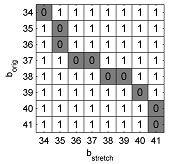
\includegraphics[scale=.5]{graph/ATAA_feature_training}}
                        \end{figure}
                    }
                    \only<4>{
                        \begin{figure}
                            \centerline{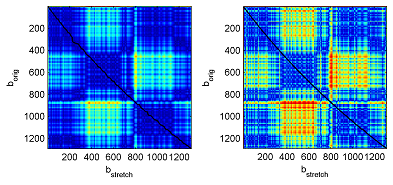
\includegraphics[scale=.5]{graph/ATAA_simmatrix_compare}}
                        \end{figure}
                    }
            \end{itemize}
        \end{frame}
        
        \begin{frame}{audio-to-audio alignment}{results}
            \begin{figure}
                \centerline{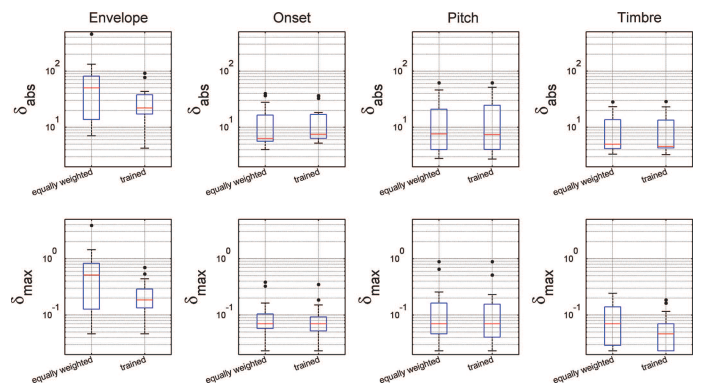
\includegraphics[scale=.5]{graph/ATAA_results}}
            \end{figure}
                \vspace{-10mm}
                \begin{columns}
                    \column{.5\linewidth}
                        \begin{itemize}
                            \item   left: instrumental
                            \item   right: a capella
                        \end{itemize}
                        \vspace{5mm}
                    \column{.25\linewidth}
                        \begin{figure}
                            \includeaudio{originals_splanky}
                        \end{figure}\vspace{-8mm}
                        \begin{center}originals\end{center}

                    \column{.25\linewidth}
                    \begin{figure}
                        \includeaudio{synced_splanky}
                    \end{figure}\vspace{-8mm}
                    \begin{center}synced\end{center}
                \end{columns}
        \end{frame}
        
    \section[A2S]{Audio to score alignment}
        \begin{frame}{audio-to-score alignment}{overview}
            \begin{itemize}
                \item   \textbf{objective}
                    \begin{itemize}
                        \item align an audio sequence with a score sequence
                    \end{itemize}
                \bigskip
                \item<2->   \textbf{use cases}
                    \begin{itemize}
                        \item   score viewer
                        \item   music education
                        \item   identify matching score/audio via cost function
                        \item   musicological analysis
                    \end{itemize}
                \bigskip
                \item<3->   \textbf{processing steps}
                    \begin{itemize}
                        \item   see audio-to-audio alignment
                    \end{itemize}
            \end{itemize}
        \end{frame}
        \begin{frame}{audio-to-score alignment}{challenges}
            \begin{itemize}
                \item   features from \textbf{different domains} (no timbre and proper loudness information in the score)
                    \begin{itemize}
                        \item   \textit{approach 1}: convert score into audio-like representation
                            \begin{itemize}
                                \item   MIDI-to-audio
                                \item   use model for harmonics and ADSR
                            \end{itemize}
                        \item   \textit{approach 2}: convert audio into score-like representation
                            \begin{itemize}
                                \item   audio-to-MIDI 
                                \item   pitch chroma
                                \item   event-based segmentation
                            \end{itemize}
                    \end{itemize}
                \bigskip
                \item<2->   pauses and rests
                    \begin{itemize}
                        \item   DTW algorithm has no graceful way of dealing with pauses
                    \end{itemize}
            \end{itemize}
        \end{frame}



    \section[summary]{lecture summary}
        \begin{frame}{summary}{lecture content}
            \begin{enumerate}
                \item   how can DTW be used to measure the similarity between two sequences
                \smallskip
                \item<2->   name possibilities of increasing the performance of DTW
                \smallskip
                \item<3->   why has DTW been suitable for speaker and keyword recognition
                \smallskip
                \item<4->   what are the main differences and commonalities between audio-to-audio and audio-to-score alignment
            \end{enumerate}
        \end{frame}
\end{document}

